\documentclass{../includes/TechDoc}
\usepackage[T1]{fontenc}
\usepackage[utf8]{inputenc}
%\usepackage[pdftex]{graphicx}
\DeclareGraphicsRule{*}{mps}{*}{}
\documentclass[12pt]{article}
\usepackage{tabularx}
\usepackage{listings}
\usepackage[russian,british]{babel}
\usepackage[utf8]{inputenc}
\setcounter{tocdepth}{3}

\renewcommand{\cftsecleader}{\cftdotfill{\cftdotsep}}

\newcommand{\intro}[1]{
    \stepcounter{section}
    \section*{\hfillПРИЛОЖЕНИЕ \arabic{section}}
    \begin{center}
        \Large\bf{#1}
    \end{center}
    \markboth{\MakeUppercase{#1}}{}
    \addcontentsline{toc}{section}{Приложение \arabic{section}. #1}
}

\lstset{basicstyle=\ttfamily,
    showstringspaces=false,
    commentstyle=\color{red},
    keywordstyle=\color{blue}
}

\title{Приложение для совместного просмотра фильмов}
\author{Студент группы БПИ-194}{В. А. Анненков}
\academicTeacher{Старший преподаватель департамента программной инженерии факультета компьютерных наук}{А. В. Поповкин}

\documentTitle{Пояснительная записка}
\documentCode{RU.17701729.02.07-01 81 01-1}

\begin{document}
    \maketitle

    \begin{abstract}
        В данном программном документе приведена пояснительная записка к серверному приложению <<Приложение для совместного просмотра фильмов>>.

        В данный документ внесены разделы «Введение», «Назначение и область применения программы», «Технические характеристики», «Ожидаемые технико-экономические показатели», «Источники, использованные при разработке».

        В разделе «Введение» указано наименование программы и документы, на основании которых ведется разработка.

        В разделе «Назначение и область применения» указано функциональное назначение программы и эксплуатационное назначение программы.

        В разделе «Технические характеристики» указаны постановка задачи на разработку программы, описание и обоснование метода организации входных и выходных данных, описание и обоснование выбора состава технических и программных средств.

        В разделе «Ожидаемые технико-экономические показатели» указана предполагаемая потребность и экономические преимущества разработки по сравнению с отечественными и зарубежными образцами или аналогами

        Настоящий документ разработан в соответствии с требованиями:
        \begin{enumerate}
            \item ГОСТ 19.101-77 Виды программ и программных документов [3];
            \item ГОСТ 19.102-77 Стадии разработки [4];
            \item ГОСТ 19.103-77 Обозначения программ и программных документов [5];
            \item ГОСТ 19.104-78 Основные надписи [6];
            \item ГОСТ 19.105-78 Общие требования к программным документам [7];
            \item ГОСТ 19.106-78 Требования к программным документам, выполненным печатным способом [8];
            \item ГОСТ 19.404-79 Пояснительная записка.
            Требования к содержанию и оформлению [9].
        \end{enumerate}
        Изменения к Пояснительной записке оформляются согласно ГОСТ 19.603-78 [10], ГОСТ 19.604-78 [11].
    \end{abstract}

    \newpage

    \tableofcontents


    \section{Введение}

    \subsection{Наименование программы}

    \subsubsection{Наименование программы на русском языке}

    Приложение для совместного просмотра фильмов.

    \subsubsection{Наименование программы на английском языке}

    Application for Collective Movie Watching.

    \subsection{Основание для разработки}

    Основанием для разработки является учебный план подготовки бакалавров по направлению 09.03.04 ``Программная инженерия'' и утвержденная академическим руководителем тема курсового проекта.


    \section{Назначение и область применения}

    \subsection{Функциональное назначение}

    Функциональным назначением <<приложения для совместного просмотра фильмов>> является предоставление пользователям возможности смотреть фильмы на расстоянии.
    Пользователи могут загружать видео на сервер, воспроизводить видео, общаться с другими пользователями посредством сообщений и <<реакций>>.

    Сама программа реализует серверную часть сервиса для совместного просмотра фильмов.
    Основная задача программы -- предоставить приложениям-клиентам всю необходимую информацию для реализации логики совместного просмотра фильмов.

    Отдельный клиент может загрузить видео на сервер, после чего любой из посторонних клиентов сможет скачать это видео.
    Для синхронизации воспроизведения видео клиенты могут использовать WebSocket интерфейс сервера.

    Каждое загруженное на сервер видео обрабатывается и разделяется на небольшие фрагменты по 10 секунд.
    Такой подход позволяет клиентам быстрее скачивать видео небольшими порциями, а также мгновенно переключаться между различными разрешениями в процессе просмотра.

    Видео преобразовывается в формат HLS (HTTP Live Streaming).
    Особенность этого формата в том, что он поддерживается любыми операционными системами: Windows, macOS, Android, iOS и т. д.
    Несмотря на то, что обработка видео в формат HLS требует длительного времени, с текущим форматом это не является проблемой.
    Видео, которые преобразованы в HLS лишь частично, могут быть воспроизведены клиентами до момента последнего обработанного фрагмента.
    Таким образом клиенты могут воспроизводить фильмы мгновенно после загрузки на сервер, не дожидаясь полной обработки.
    Обработка идёт параллельно.

    \subsection{Эксплуатационное назначение}

    Сервер может быть использован frontend-клиентами для реализации логики совместного просмотра фильмов.

    <<Приложение для совместного просмотра фильмов>> может быть использовано пользователями для совместного просмотра фильмов или других видео на расстоянии.
    Данное приложение становится особенно актуальным, когда требуется что-то посмотреть наиболее простым способом.
    Для этого в приложении реализован минималистичный интерфейс, возможность быстро загрузить собственный файл с фильмом и сразу же начать его просмотр.
    Приложение не ограничивает пользователя собственной базой фильмов, предоставляя пользователю возможность самостоятельно загружать файлы с фильмами.


    \section{Технические характеристики}

    \subsection{Постановка задачи}

    Программа обеспечивает возможность выполнения следующих функций:
    \begin{enumerate}
        \item Загрузка видеофайла для его дальнейшей обработки в формат HLS.
        \item Корректное получение обработанного видео в формате HLS.
        \item Получение актуальных данных о перемотке видео с других клиентов.
        Поддержание видео в актуальном состоянии.
        \item Получение актуальных данных о сообщениях в чате.
        \item Получение актуальных данных о <<реакциях>>.
    \end{enumerate}

    Сервер разработан на базе микросервисной архитектуры со следующими сервисами:
    \begin{enumerate}
        \item \emph{Main Service} -- Отвечает за базовое взаимодействие с клиентами.
        В основном, с помощью протокола WebSocket.
        Передаёт сообщения в чат, передаёт <<реакции>>, синхронизирует видео между клиентами.
        \item \emph{Video Service} -- Отвечает за обработку входящих видеофайлов и их хранение.
        Преобразует в формат HLS.
        Предоставляет API для работы с файлами видео.
        \item \emph{Eureka Server} -- Отвечает за взаимодействие сервисов друг с другом, помогает различным сервисам находить друг друга.
        \item \emph{Gateway Server} -- Каждый сервис работает на собственном порте.
        Клиентам было бы неудобно искать сервисы по различным адресам, поэтому этот сервис берёт на себя такую задачу.
        Точка входа для клиента. Сервис, который перенаправляет на другие сервисы.
    \end{enumerate}

    \newpage

    \subsection{Описание алгоритма и функционирования программы}

    \subsubsection{Описание алгоритма загрузки и обработки видеофайла}

    На серверной части реализован алгоритм по преобразованию единого видеоролика в набор видеороликов меньшей длительности (сегментов).
    Также добавлена конвертацию видеоролика в видеоролики с меньшим качеством (Рис.~\ref{fig:server_converting}).

    Алгоритм конвертации видеоролика следующий:
    \begin{enumerate}
        \item Клиент загружает видеофайл на сервер.
        \item Сервер конвертирует видеофайл в видеофайлы меньших разрешений.
        \[ video1080 \Rightarrow videos = \{ video1080, video720, video480, video360, video240, video144 \} \]
        Данное действие требуется сделать для обеспечения возможности менять качество воспроизводимых роликов в плеере клиента,
        а также для сжатия самих файлов с целью ускорения кэширования видеороликов клиентом.
        \item Сервер разделяет каждый видеоролик из множества видеороликов \(videos\) на небольшие фрагменты (1 сек.).
        \[ video = part1 + part2 + \cdots, \;\;\; video \in videos \]
        Данное действие требуется сделать для обеспечения возможности измененять качество и настройки видео в процессе его воспроизведения
        (без повторного кэширования и приостановки воспроизведения).
    \end{enumerate}

    Реализовано API, с помощью которого клиенты могут загружать видео на обработку (Рис.~\ref{fig:video_upload}), а затем скачивать в обработанном формате.
    Формат получаемого видео -- \emph{HLS}. Данный формат представляет из себя набор файлов: один файл формата \emph{.m3u8}, несколько файлов формата \emph{.ts}.
    Файл \emph{.m3u8} содержит в себе информацию о нахождении сегментов.
    На основе информации из файла \emph{.m3u8} клиенты делают запросы на сервер для получения требуемых сегментов.

    Сам процесс обработки реализован с помощью инструмента \emph{ffmpeg}.
    \emph{ffmpeg} -- мощный консольный инструмент, который позволяет осуществлять различные действия с видеофайлами.
    В том числе осуществлять конвертацию в различные форматы.

    \begin{lstlisting}[language=bash,caption={Пример команды ffmpeg для генерации файла в формате HLS}]
    ffmpeg -i /path/ \
         -c:a aac \
         -strict experimental \
         -c:v libx264 \
         -s filename \
         -aspect 16:9 \
         -f hls \
         -hls_list_size 0 \
         -hls_time 10 \
         -threads 0 \
         {some}p/video.m3u8
    \end{lstlisting}

    \emph{ffmpeg} это консольный инструмент, а взаимодействие с ним требуется осуществлять с помощью Java.
    Для реализации взаимодействия с bash-консолью используется класс \emph{ProcessBuilder} в Java.
    В отдельном потоке происходит чтение прогресса обработки из консоли, результат парсится с помощью регулярных выражений и преобразуется в удобный для использования формат.
    В процессе обработки клиент уже может загружать обработанные фрагменты и показывать фильм для пользователей.

    \begin{figure}[h]
        \centering
        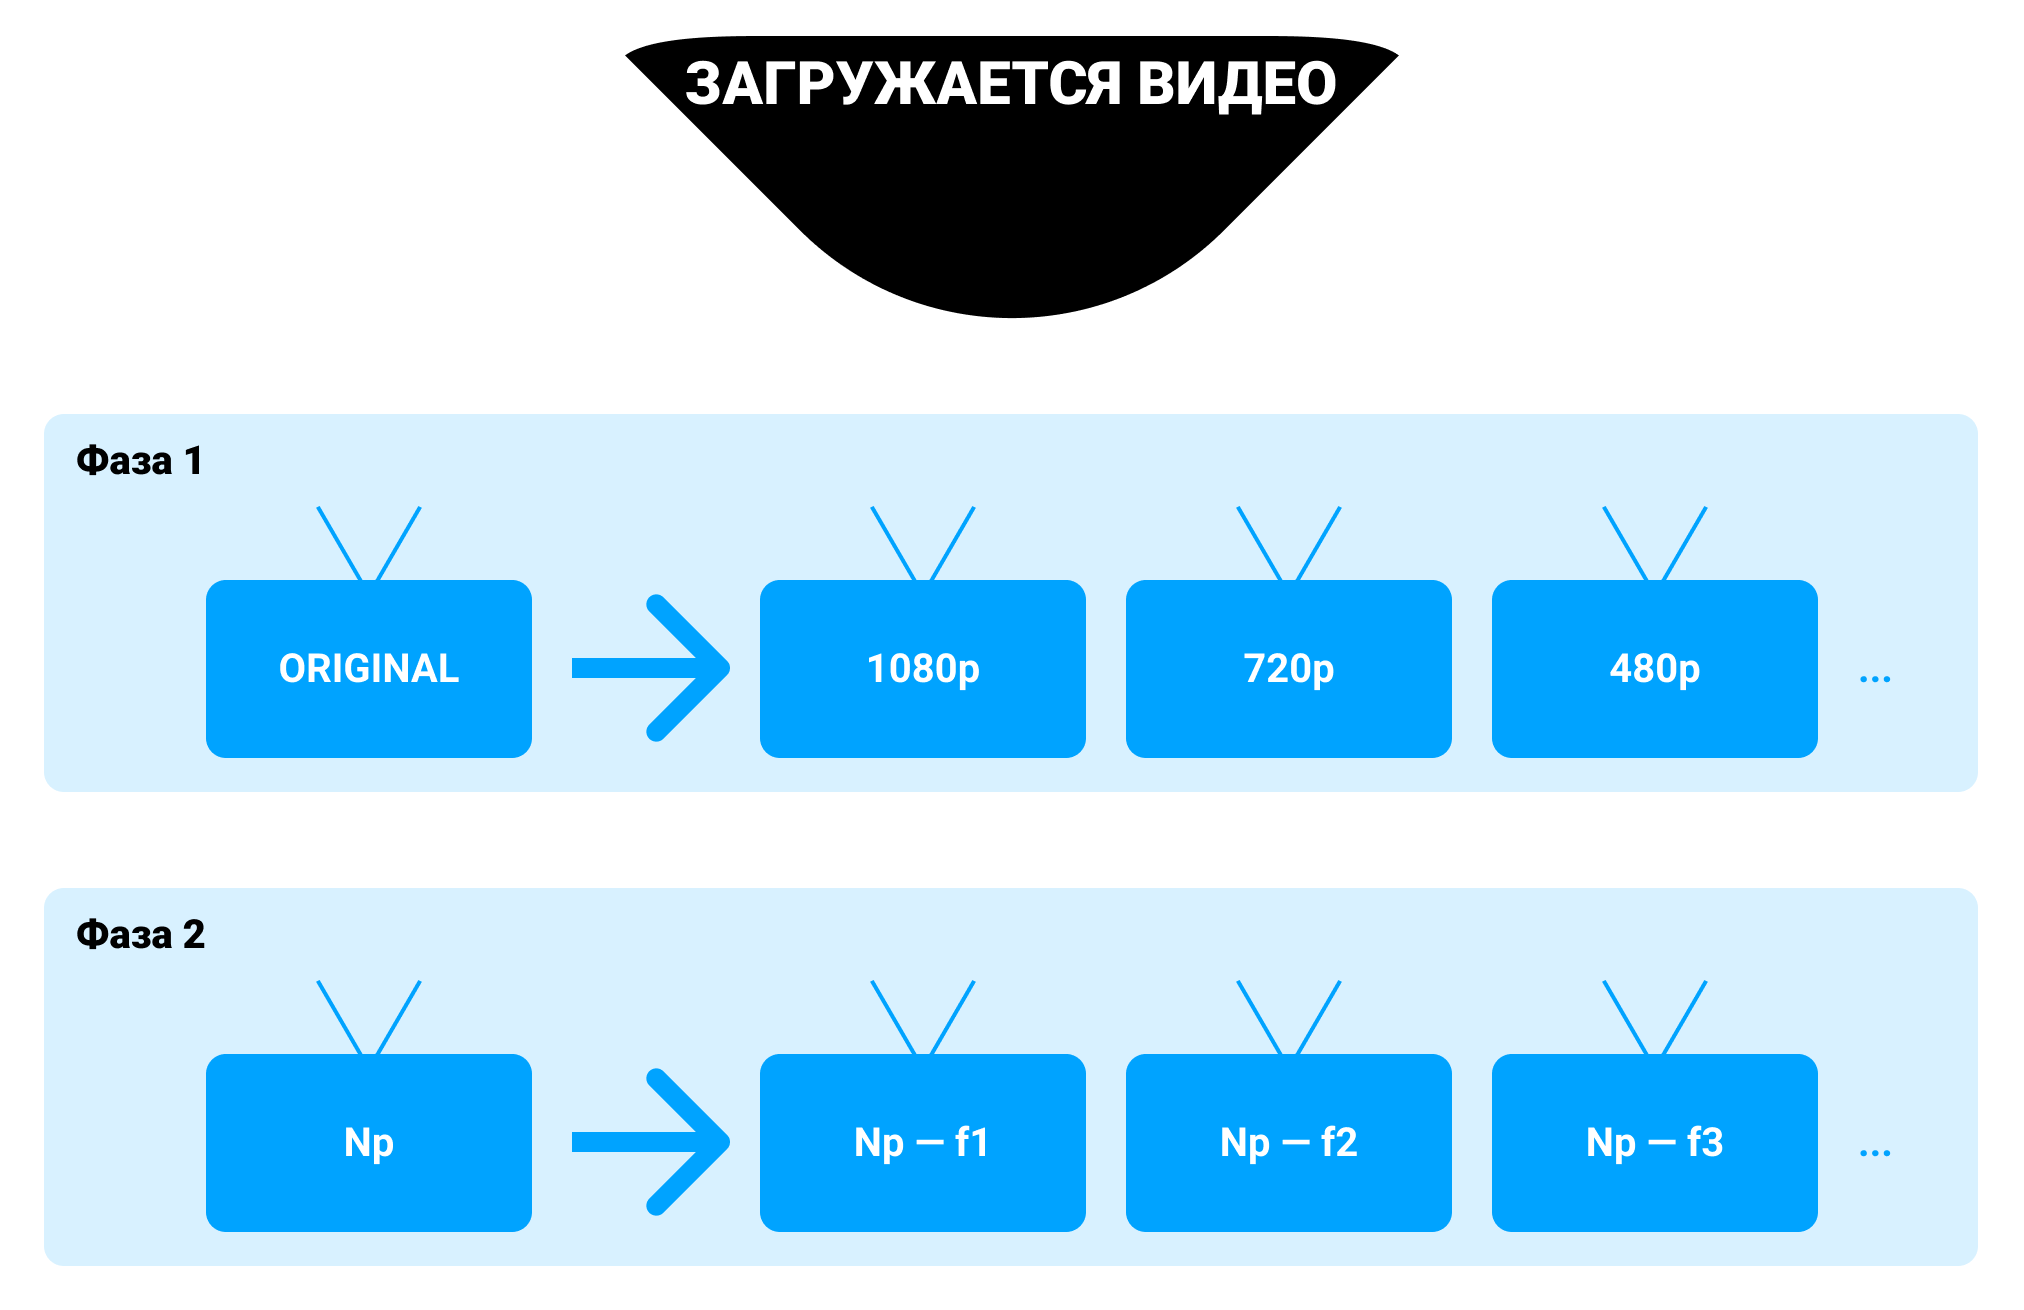
\includegraphics[width=1\linewidth]{images/server_converting.png}
        \caption{Конвертация видео в формат HLS}
        \label{fig:server_converting}
    \end{figure}

    \begin{figure}[h]
        \centering
        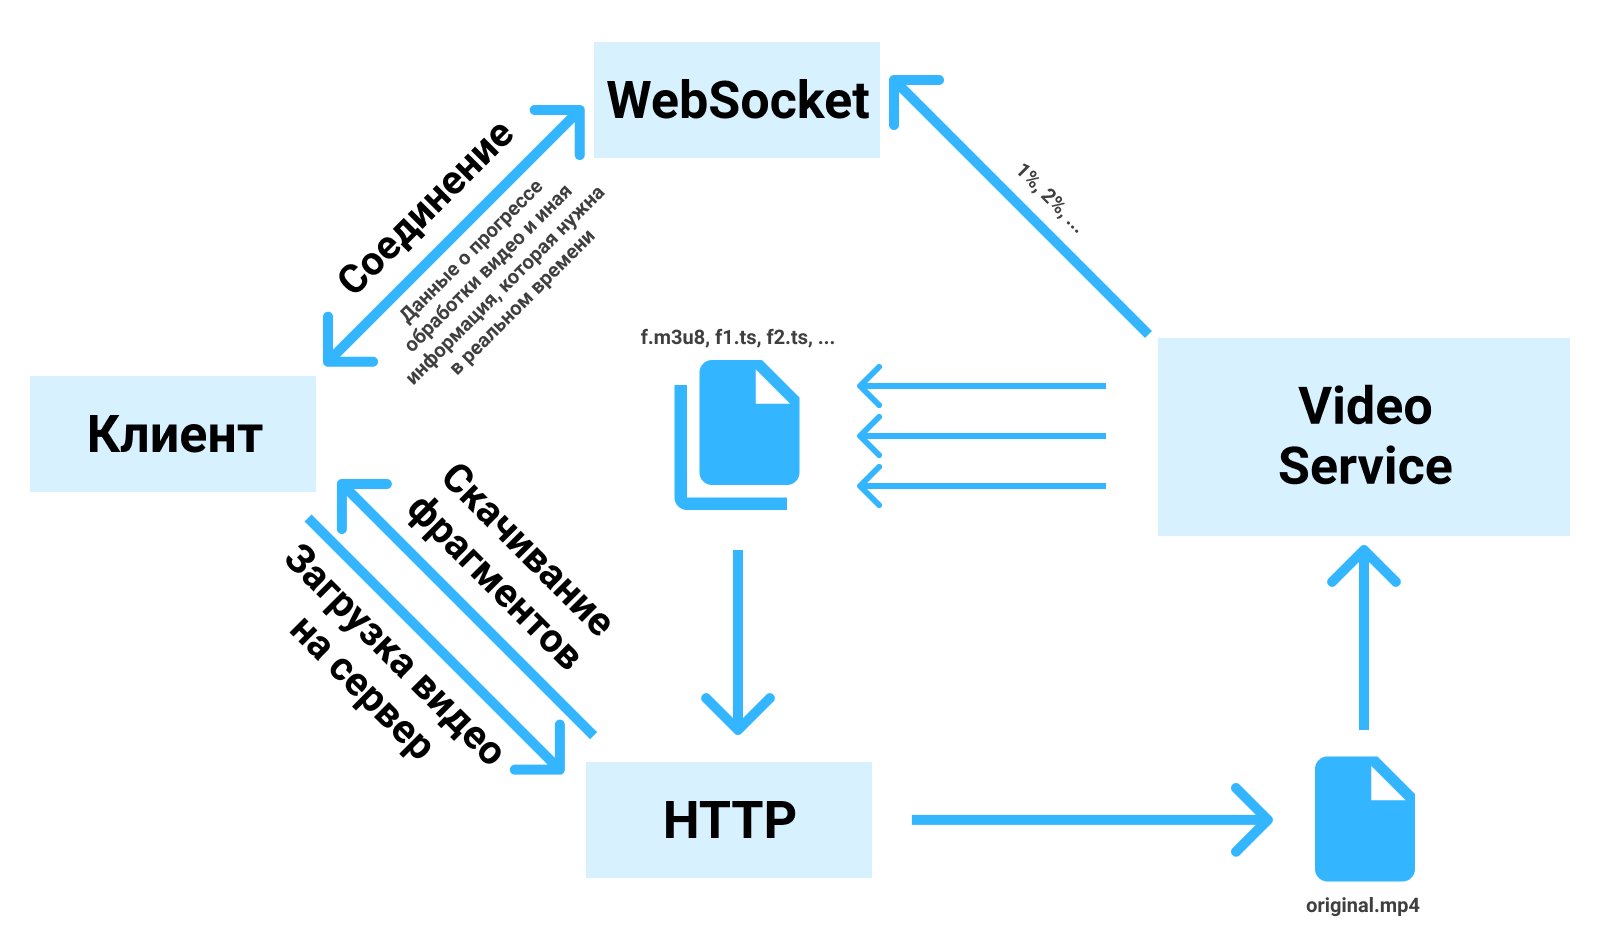
\includegraphics[width=1\linewidth]{images/video_upload.png}
        \caption{Взаимодействие клиента с сервером}
        \label{fig:video_upload}
    \end{figure}

    \subsubsection{Описание алгоритма синхронизации видеопотока}

    \paragraph{Общий алгоритм}

    Для синхронизации видеопотока между разными клиентами используется протокол WebSocket.
    Каждому клиенту требуется установить соединение с WebSocket сервером по адресу <</main/ws>>.
    В процессе просмотра видео клиенты могут отправлять следующие запросы на сервер: воспроизведение, пауза, перемотка.
    В ответ сервер отправляет данный запрос всем клиентам, просматривающим видео в текущей комнате.

    Когда сервер отправляет команду на воспроизведение, паузу или перемотку, он дополнительно передаёт информацию о времени, когда было осуществлено действие.
    Клиент может использовать эту информацию, чтобы рассчитать разницу между текущим и полученным временем, тем самым ещё сильнее уменьшив задержку при получении команды.

    В процессе перемотки видео может возникнуть ситуация, когда у разных клиентов видео загружается с различной скоростью.
    В таком случае произойдёт рассинхронизация видео, ведь некоторые клиенты запустят воспроизведение раньше остальных.
    Для решения этой ситуации была реализована перемотка с подтверждением. Алгоритм следующий:

    \begin{enumerate}
        \item Один из клиентов осуществляет перемотку видео на определённую позицию и отправляет команду для перемотки на сервер.
        \item Эту команду получают остальные клиенты и тоже осуществляют перемотку на полученную позицию.
        \item Как только некий клиент загрузил фрагмент видео и способен его воспроизвести, он отправляет на сервер команду \emph{ready}, но воспроизведение видео не начинает. Так поступают все клиенты.
        \item Когда сервер получает команду \emph{ready} от всех клиентов, он снова посылает команду всем клиентам с пометкой, что можно запускать видео.
        \item В итоге: клиенты синхронизированы и запускают видео одновременно.
    \end{enumerate}

    \paragraph{Определение задержки}

    В целях обеспечения наименьшей рассинхронизации видеопотока между клиентами, требуется хранить переменные \(diff\_sc\) и \(diff\_cs\) для
    каждого клиента.
    Данные переменные будут содержать в себе информацию о количестве затрачиваемого времени при передаче данных от сервера к клиенту или от клиента к серверу.

    Формула для определения переменных \(diff\_sc\) и \(diff\_cs\): \begin{gather*}
                                                                        diff\_sc = time\_sc_2 - time\_sc_1\\
                                                                        diff\_cs = time\_cs_2 - time\_cs_1
    \end{gather*}, где:
    \begin{itemize}[noitemsep]
        \item[--] \(time\_sc_1\) — время отправки сообщения сервером;
        \item[--] \(time\_sc_2\) — время получения сообщения клиентом;
        \item[--] \(diff\_sc\) — разница между временем отправки и временем получения при передаче сообщения от сервера к клиенту;
        \item[--] \(time\_cs_1\) — время отправки сообщения клиентом;
        \item[--] \(time\_cs_2\) — время получения сообщения сервером;
        \item[--] \(diff\_cs\) — разница между временем отправки и временем получения при передаче сообщения от клиента к серверу.
    \end{itemize}

    Так как возможно подключение нескольких клиентов, требуется хранить содержимое значений \(diff\_sc_i\) и \(diff\_cs_i\) для всех \(n\) клиентов.

    Алгоритм (Рис.~\ref{fig:interaction_format}) синхронизации видео единый:
    \begin{enumerate}
        \item Клиент \(k\) отправляет серверу запрос на действие \(d\) (перемотку/приостановку/возобновление) видео.
        \item Сервер отправляет всем клиентам сообщение с текущим серверным временем.
        Клиенты принимают значение и считают разницу \(diff\_sc_i\) с учётом своего времени.
        Затем клиенты отправляют посчитанную разницу времени в миллисекундах обратно серверу, а также отправляют текущее клиентское время.
        С учётом полученной информации сервер считает разницу \(diff\_cs_i\).
        \item Сервер отправляет всем клиентам команду выполнить действие \(d\) и передаёт каждому клиенту задержку \(delay_i\),
        которая считается по формуле: \[ delay_i = \max(diff\_sc_1, \ldots, diff\_sc_n) - diff\_sc_i + diff\_cs_k, \;\;\; i \in [1, \ldots, n] \]
    \end{enumerate}

    \begin{figure}[h]
        \centering
        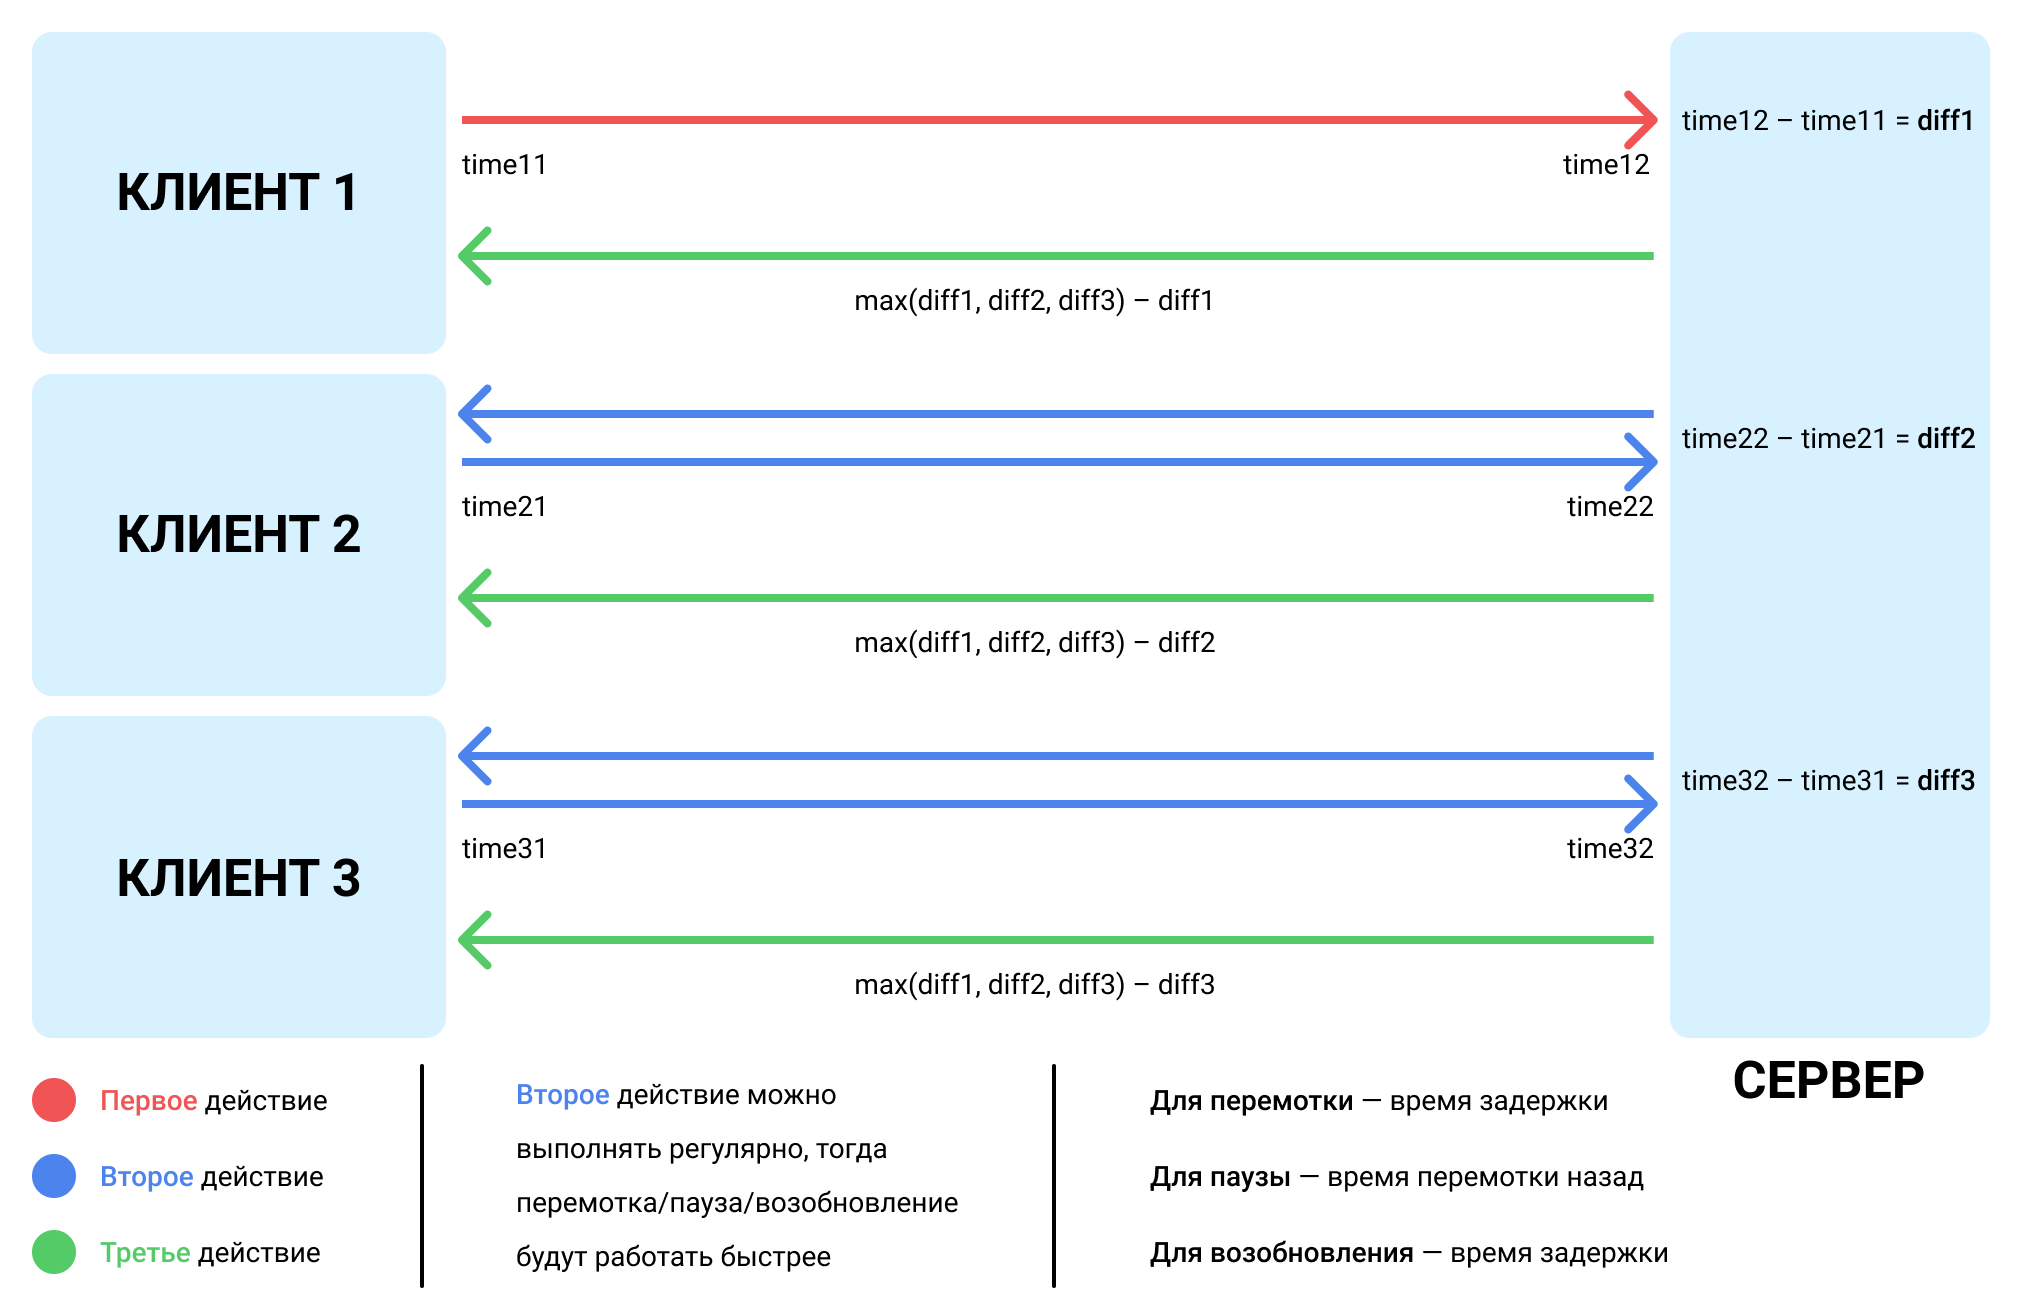
\includegraphics[width=1\linewidth]{images/interaction_format.png}
        \caption{Взаимодействие клиентов с сервером}
        \label{fig:interaction_format}
    \end{figure}

    Значение \(delay_i\) требуется по-разному использовать в различных ситуациях.
    При организации совместного просмотра фильма возможны следующие сценарии:
    \begin{itemize}
        \item[--] \textbf{Перемотка} видео на позицию \(t\) мс одним из клиентов.

        При получении такой команды все клиенты (кроме клиента-инициатора) выполняют перемотку видео на позицию \((t + delay_i)\) мс.
        \item[--] \textbf{Приостановка} видео одним из клиентов.

        При получении такой команды все клиенты (кроме клиента-инициатора) приостанавливают воспроизведение и выполняют перемотку видео на \(delay_i\) мс назад.
        \item[--] \textbf{Возобновление} видео одним из клиентов.

        При получении такой команды все клиенты (кроме клиента-инициатора) возобновляют воспроизведение и выполняют перемотку видео на \(delay_i\) мс вперёд.
    \end{itemize}

    \subsubsection{Описание алгоритма и функционирования чата и <<реакций>>}

    Реализации чата и <<реакций>> работают на основе протокола WebSocket.
    Каждому клиенту требуется установить соединение с WebSocket сервером по адресу <</main/ws>>.
    После этого клиенты могут подписаться на специальные <<топики>> комнат.
    Таким образом, когда в <<топике>> будет появляться новое действие (напр., новое сообщение или новая <<реакция>>), это действие получит любой клиент, подписанный на этот <<топик>>.

    Формат топика следующий: <</topic/room/\{\textbf{ID комнаты}\}/\{\textbf{команда}\}>>, где:
    \begin{enumerate}
        \item ID комнаты -- уникальный идентификатор комнаты, в которой клиенты просматривают фильм;
        \item команда -- тип события, на которое требуется подписаться:
        \begin{enumerate}
            \item messages -- новые сообщения;
            \item reactions -- новые <<реакции>>.
        \end{enumerate}
    \end{enumerate}

    У каждого сообщения или <<реакции>> есть информация об отправителе, которую клиенты также могут использовать.

    \clearpage

    \subsection{Описание и обоснование метода организации входных и выходных данных}

    \subsubsection{Описание и обоснование метода организации входных данных}

    Взаимодействие с клиентами организовано в виде HTTP и WebSocket подключений.

    При подключении через HTTP формат входных данных зависит от типа HTTP-метода:
    \begin{enumerate}
        \item GET -- входные данные задаются в url.
        \item POST, PUT, DELETE -- параметры задаются в теле запроса.
    \end{enumerate}

    При передаче входных данных через WebSocket формат входных данных представляет из себя JSON-объект.

    \subsubsection{Описание и обоснование метода организации выходных данных}

    При взаимодействии с любым протоколом формат выходных данных -- JSON объект.

    \subsubsection{Примеры запросов}

    \noindentОтправлен корректный запрос с видеофайлом на адрес \url{https://comnata.tv/video/upload};\\

    \noindentПолучен ответ:
    \begin{lstlisting}
    {
  		"status": "SUCCESS",
  		"videoId": "322e60eedf4245a08ebc1d9bfc23a5bd",
  		"videoUrl": "/video/getVideo/322e60eedf4245a08ebc1d9bfc23a5bd/video.m3u8"
	}
    \end{lstlisting}

    \clearpage

    \subsection{Описание и обоснование выбора состава технических и программных средств}

    \subsubsection{Состав технических и программных средств}

    Исходные коды для сервера должны реализованы с использованием следующих языков и технологий:
    \begin{enumerate}[noitemsep]
        \item Kotlin, Java -- использовать в качестве основных языков программирования;
        \item Spring Boot -- для реализации базовой архитектуры сервера, а также REST API методов и панели администрирования;
        \item Spring Flyway -- для миграций и версионирования базы данных;
        \item Hibernate, Spring Data -- для работы с базой данных, для связки таблиц базы данных с классами Java;
        \item ffmpeg -- для обработки видеофайлов: нарезка и изменение качества;
        \item PostgreSQL -- использовать в качестве СУБД;
        \item Docker, docker-compose -- для обеспечения переносимости сервера.
    \end{enumerate}

    Требования к информационным и программным характеристикам сервера:
    \begin{enumerate}[noitemsep]
        \item Наличие доступа по SSH;
        \item Открытые порты: 22, 40, 80, 443, 3000, 5432, 5454, 8080-8100;
        \item Установленные утилиты: nano, apt-get;
        \item Установленные: docker, docker-compose, docker-machine;
        \item Установленный с настройками по-умолчаию: Nginx, пользователь с доступом по SSH должен иметь права
        на редактирование конфигурации;
        \item Операционная система Ubuntu 16.04.
    \end{enumerate}

    \subsubsection{Обоснование выбора состава технических и программных средств}

    За основу веб-сервера были выбраны языки программирования Kotlin/Java и фреймворк Spring Boot.

    Kotlin и Java -- богатые по функционалу и производительные языки программирования, которые удобно использовать для написания больших приложений.
    Основным преимуществом этих языков является хорошая реализация ООП парадигмы и статическая типизация.
    Таким образом, в масштабных проектах легче отлаживать ошибки с использованием этих языков программирования.

    Spring Boot -- основной веб-фреймворк для языков программирования Kotlin и Java.
    Данный фреймворк предоставляет собственную удобную реализацию процесса IoC (Inversion of Control), благодаря которому мы можем логично выстраивать зависимости между классами внутри нашего приложения.

    Для версионирования базы данных был выбран инструмент Flyway.
    Благодаря Flyway в проекте есть возможность изменять базу данных и осуществлять переносимость её структуры.

    Spring Data позволяет удобно взаимодействовать с базой данных.
    Данный инструмент позволяет помечать аннотацией @Entity классы данных, чтобы связать их с сущностью в базе данных.
    Взаимодействие с базой производится с помощью самописных интерфейсов, реализующих интерфейс JpaRepository.

    ffmpeg -- мощный консольный инструмент для обработки видео.
    ffmpeg позволяет конвертировать видео в любой формат, добавлять аудиодорожки, менять разрешение и многое другое.
    Данный инструмент лежит в основе реализации конвертации видео в формат HLS.

    В качестве СУБД была выбрана система PostgreSQL\@.
    Такое решение было принято по нескольким причинам:
    \begin{enumerate}
        \item открытый исходный код СУБД, что делает её бесплатной;
        \item адаптированность для хранения и обработки больших объёмов данных;
        \item хорошая поддержка фреймворком Spring Data;
        \item возможность получить бесплатную базу данных PostgreSQL в админ-панели Heroku.
    \end{enumerate}

    Так как сервер написан на микросервисной архитектуре, то полезно настроить контейнер Docker, чтобы переносимость сервера была безболезненной.
    К каждому сервису написан Dockerfile, который можно запустить одной командой для запуска его контейнера Docker.
    Для связки всех контейнеров Docker используется файл docker-compose, который объединяет все Dockerfile и задаёт правила для их взаимодействия.


    \section{Ожидаемые технико-экономические показатели}

    \subsection{Предполагаемая потребность}

    Приложение могут использовать пользователи для совместного просмотра фильмов дистанционно.

    \subsection{Экономические преимущества по сравнению с отечественными и зарубежными аналогами}

    Большинство существующих сервисов поддерживают воспроизведение видео из существующей базы, не предоставляя пользователям возможность смотреть любые желаемые видео.
    Кроме того, сервисы, которые всё-таки имеют возможность загрузки видео, не позволяют просматривать видео в процессе его обработки -- для просмотра требуется дождаться полной обработки, а этот процесс может быть длительным.

    \clearpage


    \section{Источники, использованные при разработке}

    \begin{enumerate}
        \item ГОСТ 19.101-77 Виды программ и программных документов. // Единая система программной документации. – М.: ИПК Издательство стандартов, 2001.
        \item ГОСТ 19.102-77 Стадии разработки. // Единая система программной документации. – М.: ИПК Издательство стандартов, 2001.
        \item ГОСТ 19.103-77 Обозначения программ и программных документов. // Единая система программной документации. – М.: ИПК Издательство стандартов, 2001
        \item ГОСТ 19.104-78 Основные надписи. // Единая система программной документации. – М.: ИПК Издательство стандартов, 2001.
        \item ГОСТ 19.105-78 Общие требования к программным документам. // Единая система программной документации. – М.: ИПК Издательство стандартов, 2001.
        \item ГОСТ 19.106-78 Требования к программным документам, выполненным печатным способом. // Единая система программной документации. – М.: ИПК Издательство стандартов, 2001
        \item ГОСТ 19.404-79 Пояснительная записка. Требования к содержанию и оформлению. // Единая система программной документации. – М.: ИПК Издательство стандартов, 2001.
        \item Загрузка файлов [Электронный ресурс] / Spring-Projects. Режим доступа: \url{https://spring-projects.ru/guides/uploading-files/}, свободный. (Дата обращения: 15.05.2020)
        \item Как установить и настроить PostgreSQL в MacOS [Электронный ресурс] / 900913. Режим доступа: \url{https://900913.ru/note/b/postgresql-macos-9da176/}, свободный. (Дата обращения: 15.05.2020)
        \item Курс по Spring / ВТБ // [Электронный ресурс]: Google Drive. Режим доступа: \url{https://drive.google.com/drive/folders/1PQspMs1gm8aIFNua9l-wDsjgPxidqfhC}, свободный. (Дата обращения: 15.05.2021)
        \item Тянем ролик с Youtube и раздаем по WebRTC в реалтайме [Электронный ресурс] / Flashphoner. Режим доступа: \url{https://flashphoner.com/tyanem-rolik-s-youtube-i-razdaem-po-webrtc-v-realtajme/?lang=ru}, свободный. (Дата обращения: 15.05.2020)
        \item Adaptive HTTP Streaming Technologies: HLS vs. DASH / Tech Blog // [Электронный ресурс]: StriveCast. Режим доступа: \url{https://strivecast.com/hls-vs-mpeg-dash/}, свободный. (Дата обращения: 15.05.2021)
        \item Create Multiple tables [Электронный ресурс] / LaunchSchool. Режим доступа: \url{https://launchschool.com/books/sql_first_edition/read/multi_tables}, свободный. (Дата обращения: 15.05.2020)
        \item Docker документация [Электронный ресурс] / Docker. Режим доступа: \url{https://docs.docker.com/}, свободный. (Дата обращения: 15.05.2020)
        \item ffmpeg документация [Электронный ресурс] / ffmpeg. Режим доступа: \url{https://ffmpeg.org/ffmpeg.html}, свободный. (Дата обращения: 15.05.2020)
        \item GitHub [Электронный ресурс]. Режим доступа: \url{https://github.com/}, свободный. (Дата обращения: 15.05.2020)
        \item How do I use ffmpeg to get the video resolution? / Vladimir Stazhilov // [Электронный ресурс]: SuperUser. Режим доступа: \url{https://superuser.com/questions/841235/how-do-i-use-ffmpeg-to-get-the-video-resolution}, свободный. (Дата обращения: 15.05.2021)
        \item How to create .mpd or .m3u8 video file on the server using FFMPEG for Adaptive Streaming / Mayur Solanki // [Электронный ресурс]: Medium. Режим доступа: \url{https://mayur-solanki.medium.com/how-to-create-mpd-or-m3u8-video-file-from-server-using-ffmpeg-97e9e1fbf6a3}, свободный. (Дата обращения: 15.05.2021)
        \item How to read ffmpeg response from java and use it to create a progress bar? / shalki // [Электронный ресурс]: StackOverflow. Режим доступа: \url{https://stackoverflow.com/questions/10927718/how-to-read-ffmpeg-response-from-java-and-use-it-to-create-a-progress-bar}, свободный. (Дата обращения: 15.05.2021)
        \item How video streaming works on the web: An introduction / Paul Berberian // [Электронный ресурс]: Medium. Режим доступа: \url{https://medium.com/canal-tech/how-video-streaming-works-on-the-web-an-introduction-7919739f7e1}, свободный. (Дата обращения: 15.05.2021)
        \item Kotlin документация [Электронный ресурс] / JetBrains. Режим доступа: \url{https://kotlinlang.org/docs/}, свободный. (Дата обращения: 15.05.2020)
        \item PostgreSQL документация [Электронный ресурс] / PostgreSQL. Режим доступа: \url{https://www.postgresql.org/docs/}, свободный. (Дата обращения: 15.05.2020)
        \item Spring документация [Электронный ресурс] / Spring. Режим доступа: \url{https://spring.io/}, свободный. (Дата обращения: 15.05.2020)
        \item Spring Cloud Demo Project / gonwan // [Электронный ресурс]: GitHub. Режим доступа: \url{https://github.com/gonwan/spring-cloud-demo}, свободный. (Дата обращения: 15.05.2021)
        \item Spring Cloud Netflix Microservices -- start project (серия статей) -- часть 4 / Kirill Sereda // [Электронный ресурс]: Medium. Режим доступа: \url{https://medium.com/@kirill.sereda/spring-cloud-netflix-microservices-start-project-%D1%81%D0%B5%D1%80%D0%B8%D1%8F-%D1%81%D1%82%D0%B0%D1%82%D0%B5%D0%B9-%D1%87%D0%B0%D1%81%D1%82%D1%8C-4-d2137d19d783}, свободный. (Дата обращения: 15.05.2021)
        \item StackOverflow [Электронный ресурс]. Режим доступа: \url{https://stackoverflow.com/}, свободный. (Дата обращения: 15.05.2020)
        \item streaming an mkv file while processing with ffmpeg / Phani Rithvij // [Электронный ресурс]: StackOverflow. Режим доступа: \url{https://stackoverflow.com/questions/55460359/streaming-an-mkv-file-while-processing-with-ffmpeg}, свободный. (Дата обращения: 15.05.2021)
    \end{enumerate}

    \clearpage
    \appendix

    \intro{Терминология}

    \noindent
    \textbf{IoC (Inversion of Control)} -- архитектурный принцип объектно-ориентированного программирования, используемый для уменьшения зацепления (связанности) в компьютерных программах.\\\\
    \textbf{HLS (HTTP Live Streaming)} -- коммуникационный протокол для потоковой передачи медиа на основе HTTP, разработанный компанией Apple.\\\\
    \textbf{База данных} -- совокупность данных, хранимых в соответствии со схемой данных, манипулирование которыми выполняют в соответствии с правилами средств моделирования данных.\\\\
    \textbf{Реакция} -- всплывающий смайлик для быстрой передачи эмоций во время просмотра.\\\\
    \textbf{Терминал} -- разновидность текстового интерфейса между человеком и компьютером, в котором инструкции компьютеру даются в основном путём ввода с клавиатуры текстовых строк (команд).\\\\
    \textbf{Комната} -- виртуальное пространство, в котором воспроизводится видео и к которому могут подключаться пользователи.\\\\
    \textbf{Клиент} -- приложение, которое подключается к серверу.\\\\
    \textbf{Сегмент} -- небольшой отрывок из исходного видео.\\\\
    \textbf{Сервер} -- выделенный или специализированный компьютер для выполнения сервисного программного обеспечения.\\\\
    \textbf{Серверное приложение} -- программа на сервере.\\\\
    \textbf{СУБД} -- система управления базами данных.\\\\
    \textbf{Фреймворк} -- дополнение к программе, расширяющее функционал или упрощающее процесс разработки.\\\\

    \intro{Описание формата HLS}

    Формат HLS представляет из себя набор файлов с расширениями \emph{.m3u8} (один файл) и \emph{.ts} (несколько файлов).

    \begin{itemize}
        \item[--] \emph{.m3u8} -- Обычный текстовый файл, который содержит информацию о расположении файлов с расширением \emph{.ts}.
        Может ссылаться как на медиа-файлы, так и на другие файлы с расширением \emph{.m3u8}.
        Например, для указания разрешений видео.
        \item[--] \emph{.ts} -- Медиа-файл, небольшой отрывок из исходного видео.
    \end{itemize}

    \begin{lstlisting}[language=text,caption={Пример содержимого файла с расширением .m3u8}]
    #EXTM3U
	#EXT-X-VERSION:3
	#EXT-X-TARGETDURATION:17
	#EXT-X-MEDIA-SEQUENCE:0
	#EXTINF:16.683333,
	video0.ts
	#EXTINF:8.341667,
	video1.ts
	#EXTINF:8.341667,
	video2.ts
	#EXTINF:8.341667,
	video3.ts
	...
    \end{lstlisting}

    \intro{Структура базы данных}

    Приведена схема базы данных (Рис.~\ref{fig:db_scheme}).

    В базе данных:
    \begin{itemize}
        \item[--] таблица \emph{app\_user} хранит информацию о пользователях;
        \item[--] таблица \emph{room} хранит информацию о комнатах;
        \item[--] таблица \emph{flyway\_schema\_history} хранит информацию о применённых миграциях к базе данных.
    \end{itemize}

    \begin{figure}[h]
        \centering
        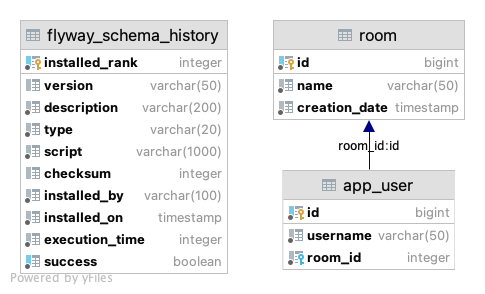
\includegraphics[width=0.5\linewidth]{images/db_scheme.png}
        \caption{Схема базы данных}
        \label{fig:db_scheme}
    \end{figure}

    \intro{Описание и функциональное назначение классов}

    \begin{table}[h]
        \caption{\label{tab:class-AuthConfirmView-table}Описание классов модуля MainService}
        \begin{tabularx}{\textwidth}{|l|X|}
            \hline
            \textbf{Класс}           & \textbf{Назначение}                                                    \\
            \hline
            MainController              & Контроллер с основными методами                                        \\
            \hline
            WebsocketController         & Контроллер с методами для взаимодействия через протокол WebSocket      \\
            \hline
            RoomService                 & Сервис работы с комнатами                                              \\
            \hline
            WebsocketService            & Сервис для взаимодействия с WebSocket                                  \\
            \hline
            RoomRepository              & Репозиторий для получения информации о комнатах                        \\
            \hline
            UserRepository              & Репозиторий для получения информации о пользователях                   \\
            \hline
            WebsocketEventListener      & Слушатель для определения событий подключения/отключения пользователей \\
            \hline
            Room                        & Модель комнаты                                                         \\
            \hline
            User                        & Модель пользователя                                                    \\
            \hline
            RoomActionRequest           & Модель запроса для синхронизации видео                                 \\
            \hline
            RoomChatMessageRequest      & Модель запроса для сообщений в чате                                    \\
            \hline
            RoomReactionRequest         & Модель запроса для реакций                                             \\
            \hline
            Response                    & Абстрактная модель ответа                                              \\
            \hline
            RoomActionResponse          & Модель ответа для синхронизации видео                                  \\
            \hline
            RoomChatMessageResponse     & Модель ответа для сообщений в чате                                     \\
            \hline
            RoomJoinResponse            & Модель ответа для подключений к комнате                                \\
            \hline
            RoomLeftResponse            & Модель ответа для выходов из комнаты                                   \\
            \hline
            RoomReactionResponse        & Модель ответа для реакции                                              \\
            \hline
            WebsocketEnums              & Enum классы для WebSocket                                              \\
            \hline
        \end{tabularx}
    \end{table}

    \begin{table}[h]
        \caption{\label{tab:class-AuthConfirmView-table}Описание классов модуля VideoService}
        \begin{tabularx}{\textwidth}{|l|X|}
            \hline
            \textbf{Класс}           & \textbf{Назначение}                              \\
            \hline
            VideoController             & Контроллер для взаимодействия с видеофайлами     \\
            \hline
            VideoService                & Сервис для работы с видеофайлами                 \\
            \hline
            FfmpegManager               & Класс для обработки видеофайлов с помощью ffmpeg \\
            \hline
            VideoResolution             & Модель разрешения видео                          \\
            \hline
            MainClient                  & Клиент для получения информации из MainService   \\
            \hline
        \end{tabularx}
    \end{table}

    \intro{Описание и функциональное назначение полей, методов и свойств модуля MainService}

    \begin{table}[h]
        \caption{\label{tab:class-AuthConfirmView-table}Описание полей, методов и свойств класса MainController}
        \begin{tabularx}{\textwidth}{|l|l|l|l|X|}
            \hline
            \multicolumn{5}{|c|}{MainController} \\ \hline
            \multicolumn{5}{|l|}{\textbf{Поля}} \\ \hline
            \textbf{Имя} & \textbf{М. дост.} & \textbf{Тип} & \multicolumn{2}{|>{\hsize=\dimexpr2\hsize+2\tabcolsep+\arrayrulewidth\relax}X|}{\textbf{Назначение}} \\ \hline
            logger & private & Logger & \multicolumn{2}{|>{\hsize=\dimexpr2\hsize+2\tabcolsep+\arrayrulewidth\relax}X|}{Объект для логгирования} \\ \hline
            roomService & private & RoomService & \multicolumn{2}{|>{\hsize=\dimexpr2\hsize+2\tabcolsep+\arrayrulewidth\relax}X|}{Сервис для взаимодействия с комнатами} \\ \hline
            \multicolumn{5}{|l|}{\textbf{Методы}} \\ \hline
            \textbf{Имя}     & \textbf{М. дост.} & \textbf{Тип} & \textbf{Арг.}    & \textbf{Назначение}                                \\ \hline
            createVideo      & public            & void         & String videoUuid & Метод для добавления видео в базу данных           \\ \hline
            setVideoProgress & public            & void         & String videoUuid & Метод для установки прогресса обработки видеофайла \\ \hline
        \end{tabularx}
    \end{table}

    \begin{table}[h]
        \caption{\label{tab:class-AuthConfirmView-table}Описание полей, методов и свойств класса WebsocketController}
        \begin{tabularx}{\textwidth}{|p{3.2cm}|l|l|l|X|}
            \hline
            \multicolumn{5}{|c|}{WebsocketController} \\ \hline
            \multicolumn{5}{|l|}{\textbf{Поля}} \\ \hline
            \textbf{Имя} & \textbf{М. дост.} & \textbf{Тип} & \multicolumn{2}{|l|}{\textbf{Назначение}} \\ \hline
            URL\_ROOM \_JOIN & private & String & \multicolumn{2}{|l|}{Сервис для взаимодействия с комнатами} \\ \hline
            URL\_ROOM \_VIDEO \_ACTION & private & String & \multicolumn{2}{|l|}{Сервис для взаимодействия с комнатами} \\ \hline
            URL\_ROOM \_VIDEO \_ACTION \_READY & private & String & \multicolumn{2}{|l|}{Сервис для взаимодействия с комнатами} \\ \hline
            URL\_ROOM \_CHAT \_MESSAGE & private & String & \multicolumn{2}{|l|}{Сервис для взаимодействия с комнатами} \\ \hline
            URL\_ROOM \_REACTION & private & String & \multicolumn{2}{|l|}{Сервис для взаимодействия с комнатами} \\ \hline
            logger & private & Logger & \multicolumn{2}{|l|}{Объект для логгирования} \\ \hline
            roomService & private & RoomService & \multicolumn{2}{|l|}{Сервис для взаимодействия с комнатами} \\ \hline
            \multicolumn{5}{|l|}{\textbf{Методы}} \\ \hline
            \textbf{Имя}                  & \textbf{М. дост.} & \textbf{Тип} & \textbf{Арг.}       & \textbf{Назначение}                                \\ \hline
            processRoomJoin               & public            & void         & Principal principal & Метод для добавления видео в базу данных           \\ \hline
            processRoom VideoAction       & public            & void         & Principal principal & Метод для установки прогресса обработки видеофайла \\ \hline
            processRoom VideoAction Ready & public            & void         & Principal principal & Метод для установки прогресса обработки видеофайла \\ \hline
            processRoom ChatMessage       & public            & void         & Principal principal & Метод для установки прогресса обработки видеофайла \\ \hline
            processRoom Reaction          & public            & void         & Principal principal & Метод для установки прогресса обработки видеофайла \\ \hline
        \end{tabularx}
    \end{table}

    \begin{table}[h]
        \caption{\label{tab:class-AuthConfirmView-table}Описание полей, методов и свойств класса RoomService}
        \begin{tabularx}{\textwidth}{|p{3.5cm}|l|l|l|X|}
            \hline
            \multicolumn{5}{|c|}{RoomService} \\ \hline
            \multicolumn{5}{|l|}{\textbf{Поля}} \\ \hline
            \textbf{Имя} & \textbf{М. дост.} & \textbf{Тип} & \multicolumn{2}{|>{\hsize=\dimexpr2\hsize+2\tabcolsep+\arrayrulewidth\relax}X|}{\textbf{Назначение}} \\ \hline
            logger & private & Logger & \multicolumn{2}{|>{\hsize=\dimexpr2\hsize+2\tabcolsep+\arrayrulewidth\relax}X|}{Объект для логгирования} \\ \hline
            websocketService & private & RoomService & \multicolumn{2}{|>{\hsize=\dimexpr2\hsize+2\tabcolsep+\arrayrulewidth\relax}X|}{Сервис для взаимодействия с протоколом WebSocket} \\ \hline
            userRepository & private & RoomService & \multicolumn{2}{|>{\hsize=\dimexpr2\hsize+2\tabcolsep+\arrayrulewidth\relax}X|}{Сервис для взаимодействия с пользователями} \\ \hline
            roomRepository & private & RoomService & \multicolumn{2}{|>{\hsize=\dimexpr2\hsize+2\tabcolsep+\arrayrulewidth\relax}X|}{Сервис для взаимодействия с комнатами} \\ \hline
            actionsStore & private & RoomService & \multicolumn{2}{|>{\hsize=\dimexpr2\hsize+2\tabcolsep+\arrayrulewidth\relax}X|}{Компонент для хранения локальных данных} \\ \hline
            URL\_ROOM \_JOINS & private & RoomService & \multicolumn{2}{|>{\hsize=\dimexpr2\hsize+2\tabcolsep+\arrayrulewidth\relax}X|}{Константа url входов в комнату} \\ \hline
            URL\_ROOM \_LEFTS & private & RoomService & \multicolumn{2}{|>{\hsize=\dimexpr2\hsize+2\tabcolsep+\arrayrulewidth\relax}X|}{Константа url выходов из комнаты} \\ \hline
            URL\_ROOM \_ACTIONS & private & RoomService & \multicolumn{2}{|>{\hsize=\dimexpr2\hsize+2\tabcolsep+\arrayrulewidth\relax}X|}{Константа url действий с видео} \\ \hline
            URL\_ROOM \_CHAT \_MESSAGES & private & RoomService & \multicolumn{2}{|>{\hsize=\dimexpr2\hsize+2\tabcolsep+\arrayrulewidth\relax}X|}{Константа url сообщений в чате} \\ \hline
            URL\_ROOM \_REACTIONS & private & RoomService & \multicolumn{2}{|>{\hsize=\dimexpr2\hsize+2\tabcolsep+\arrayrulewidth\relax}X|}{Константа url реакций} \\ \hline
            \multicolumn{5}{|l|}{\textbf{Методы}} \\ \hline
            \textbf{Имя}                 & \textbf{М. дост.} & \textbf{Тип} & \textbf{Арг.}       & \textbf{Назначение}                   \\ \hline
            checkIsRoomExist             & public            & void         & Principal principal & Метод для проверки наличия комнаты    \\ \hline
            createRoom                   & public            & void         & Principal principal & Метод для создания комнаты            \\ \hline
            processVideoJoin             & public            & void         & Principal principal & Метод для реализации входа            \\ \hline
            processVideoLeft             & public            & void         & Principal principal & Метод для реализации выхода           \\ \hline
            processRoom VideoAction      & public            & void         & Principal principal & Метод для реализации действия с видео \\ \hline
            processRoom VideoActionSeek  & public            & void         & Principal principal & Метод для реализации перемотки        \\ \hline
            processRoom VideoActionReady & public            & void         & Principal principal & Метод для реализации готовности       \\ \hline
            processRoom ChatMessage      & public            & void         & Principal principal & Метод для реализации сообщения в чате \\ \hline
            processRoom ChatReaction     & public            & void         & Principal principal & Метод для реализации реакции в чате   \\ \hline
        \end{tabularx}
    \end{table}

    \begin{table}[h]
        \caption{\label{tab:class-AuthConfirmView-table}Описание полей, методов и свойств класса WebsocketService}
        \begin{tabularx}{\textwidth}{|l|l|l|p{3cm}|X|}
            \hline
            \multicolumn{5}{|c|}{WebsocketService} \\ \hline
            \multicolumn{5}{|l|}{\textbf{Поля}} \\ \hline
            \textbf{Имя} & \textbf{М. дост.} & \textbf{Тип} & \multicolumn{2}{|>{\hsize=\dimexpr2\hsize+2\tabcolsep+\arrayrulewidth\relax}X|}{\textbf{Назначение}} \\ \hline
            logger & private & Logger & \multicolumn{2}{|>{\hsize=\dimexpr2\hsize+2\tabcolsep+\arrayrulewidth\relax}X|}{Объект для логгирования} \\ \hline
            messagingTemplate & private & SimpMessagingTemplate & \multicolumn{2}{|>{\hsize=\dimexpr2\hsize+2\tabcolsep+\arrayrulewidth\relax}X|}{Объект для отправки WebSocket сообщений} \\ \hline
            simpUserRegistry & private & SimpUserRegistry & \multicolumn{2}{|>{\hsize=\dimexpr2\hsize+2\tabcolsep+\arrayrulewidth\relax}X|}{Объект для получения количества WebSocket сессий} \\ \hline
            \multicolumn{5}{|l|}{\textbf{Методы}} \\ \hline
            \textbf{Имя}        & \textbf{М. дост.} & \textbf{Тип} & \textbf{Арг.}                       & \textbf{Назначение}                       \\ \hline
            send                & public            & void         & url: String, obj: Any               & Метод для отправки сообщений в топик      \\ \hline
            sendToUser          & public            & void         & url: String, user: String, obj: Any & Метод для отправки сообщений пользователю \\ \hline
            getNumberOfSessions & public            & int          & -                                   & Метод для получения списка сессий         \\ \hline
        \end{tabularx}
    \end{table}

    \begin{table}[h]
        \caption{\label{tab:class-AuthConfirmView-table}Описание полей, методов и свойств класса RoomRepository}
        \begin{tabularx}{\textwidth}{|l|l|l|l|X|}
            \hline
            \multicolumn{5}{|c|}{RoomRepository} \\ \hline
            \multicolumn{5}{|l|}{\textbf{Методы}} \\ \hline
            \textbf{Имя}   & \textbf{М. дост.} & \textbf{Тип} & \textbf{Арг.} & \textbf{Назначение}                      \\ \hline
            saveAndFlush   & public            & Room         & room: Room    & Метод для сохранения комнаты в базу      \\ \hline
            findRoomByName & public            & Room?        & name: String  & Метод для поиска комнаты в базе по имени \\ \hline
        \end{tabularx}
    \end{table}

    \begin{table}[h]
        \caption{\label{tab:class-AuthConfirmView-table}Описание полей, методов и свойств класса UserRepository}
        \begin{tabularx}{\textwidth}{|l|l|l|l|X|}
            \hline
            \multicolumn{5}{|c|}{UserRepository} \\ \hline
            \multicolumn{5}{|l|}{\textbf{Методы}} \\ \hline
            \textbf{Имя}       & \textbf{М. дост.} & \textbf{Тип} & \textbf{Арг.}    & \textbf{Назначение}                           \\ \hline
            findUserByUsername & public            & User         & name: String     & Метод для поиска пользователя в базе по имени \\ \hline
            findAllByRoomName  & public            & List<User>   & roomName: String & Метод для поиска всех участников комнаты      \\ \hline
        \end{tabularx}
    \end{table}

    \begin{table}[h]
        \caption{\label{tab:class-WebsocketEventListener-table}Описание полей, методов и свойств класса WebsocketEventListener}
        \begin{tabularx}{\textwidth}{|l|l|l|p{4.3cm}|X|}
            \hline
            \multicolumn{5}{|c|}{WebsocketEventListener} \\ \hline
            \multicolumn{5}{|l|}{\textbf{Поля}} \\ \hline
            \textbf{Имя} & \textbf{М. дост.} & \textbf{Тип} & \multicolumn{2}{|>{\hsize=\dimexpr2\hsize+2\tabcolsep+\arrayrulewidth\relax}X|}{\textbf{Назначение}} \\ \hline
            logger & private & Logger & \multicolumn{2}{|>{\hsize=\dimexpr2\hsize+2\tabcolsep+\arrayrulewidth\relax}X|}{Объект для логгирования} \\ \hline
            roomService & private & RoomService & \multicolumn{2}{|>{\hsize=\dimexpr2\hsize+2\tabcolsep+\arrayrulewidth\relax}X|}{Сервис для взаимодействия с комнатами} \\ \hline
            \multicolumn{5}{|l|}{\textbf{Методы}} \\ \hline
            \textbf{Имя}            & \textbf{М. дост.} & \textbf{Тип} & \textbf{Арг.}                 & \textbf{Назначение}                       \\ \hline
            handleSessionConnect    & public            & void         & event: SessionConnectEvent    & Метод для определения события подключения \\ \hline
            handleSessionDisconnect & public            & void         & event: SessionDisconnectEvent & Метод для определения события отключения  \\ \hline
        \end{tabularx}
    \end{table}

    \begin{table}[h]
        \caption{\label{tab:class-WebsocketEventListener-table}Описание полей, методов и свойств класса Action}
        \begin{tabularx}{\textwidth}{|l|l|l|p{3cm}|X|}
            \hline
            \multicolumn{5}{|c|}{Action} \\ \hline
            \multicolumn{5}{|l|}{\textbf{Поля}} \\ \hline
            \textbf{Имя} & \textbf{М. дост.} & \textbf{Тип} & \multicolumn{2}{|>{\hsize=\dimexpr2\hsize+2\tabcolsep+\arrayrulewidth\relax}X|}{\textbf{Назначение}} \\ \hline
            id & private & Long & \multicolumn{2}{|>{\hsize=\dimexpr2\hsize+2\tabcolsep+\arrayrulewidth\relax}X|}{ID события} \\ \hline
            type & private & String & \multicolumn{2}{|>{\hsize=\dimexpr2\hsize+2\tabcolsep+\arrayrulewidth\relax}X|}{Тип события} \\ \hline
            seekTime & private & Double & \multicolumn{2}{|>{\hsize=\dimexpr2\hsize+2\tabcolsep+\arrayrulewidth\relax}X|}{Время в видео для перемотки} \\ \hline
            author & private & String & \multicolumn{2}{|>{\hsize=\dimexpr2\hsize+2\tabcolsep+\arrayrulewidth\relax}X|}{Автор события} \\ \hline
            users & private & MutableSet<String> & \multicolumn{2}{|>{\hsize=\dimexpr2\hsize+2\tabcolsep+\arrayrulewidth\relax}X|}{Пользователи, задействованные в событии} \\ \hline
            \multicolumn{5}{|l|}{\textbf{Методы}} \\ \hline
            \textbf{Имя}   & \textbf{М. дост.} & \textbf{Тип} & \textbf{Арг.}         & \textbf{Назначение}                                                    \\ \hline
            addUser        & public            & void         & user: String          & Метод для добавления пользователя в список задействованных             \\ \hline
            addUsers       & public            & void         & newUsers: Set<String> & Метод для добавления нескольких пользователей в список задействованных \\ \hline
            deleteUser     & public            & void         & user: String          & Метод для удаления пользователя из списка задействованных              \\ \hline
            deleteAllUsers & public            & void         & user: String          & Метод для удаления всех пользователей из списка задействованных        \\ \hline
        \end{tabularx}
    \end{table}

    \begin{table}[h]
        \caption{\label{tab:class-WebsocketEventListener-table}Описание полей, методов и свойств класса Room}
        \begin{tabularx}{\textwidth}{|l|l|l|X|}
            \hline
            \multicolumn{4}{|c|}{Room} \\ \hline
            \multicolumn{4}{|l|}{\textbf{Поля}} \\ \hline
            \textbf{Имя} & \textbf{М. дост.} & \textbf{Тип}  & \textbf{Назначение}          \\ \hline
            name         & public            & String        & Имя комнаты                  \\ \hline
            creationDate & public            & LocalDateTime & Дата создания комнаты        \\ \hline
            id           & public            & Long          & ID комнаты                   \\ \hline
            users        & public            & Set<User>     & Список пользователей комнаты \\ \hline
        \end{tabularx}
    \end{table}

    \begin{table}[h]
        \caption{\label{tab:class-WebsocketEventListener-table}Описание полей, методов и свойств класса User}
        \begin{tabularx}{\textwidth}{|l|l|l|X|}
            \hline
            \multicolumn{4}{|c|}{User} \\ \hline
            \multicolumn{4}{|l|}{\textbf{Поля}} \\ \hline
            \textbf{Имя} & \textbf{М. дост.} & \textbf{Тип} & \textbf{Назначение}                       \\ \hline
            username     & public            & String       & Имя пользователя                          \\ \hline
            room         & public            & Room         & Комната, к которой подключён пользователь \\ \hline
            id           & public            & Long         & ID пользователя                           \\ \hline
        \end{tabularx}
    \end{table}

    \begin{table}[h]
        \caption{\label{tab:class-WebsocketEventListener-table}Описание полей, методов и свойств класса RoomActionReadyRequest}
        \begin{tabularx}{\textwidth}{|l|l|l|X|}
            \hline
            \multicolumn{4}{|c|}{RoomActionReadyRequest} \\ \hline
            \multicolumn{4}{|l|}{\textbf{Поля}} \\ \hline
            \textbf{Имя} & \textbf{М. дост.} & \textbf{Тип} & \textbf{Назначение}                      \\ \hline
            actionId     & public            & Long?        & ID действия для подтверждения готовности \\ \hline
        \end{tabularx}
    \end{table}

    \begin{table}[h]
        \caption{\label{tab:class-WebsocketEventListener-table}Описание полей, методов и свойств класса RoomActionRequest}
        \begin{tabularx}{\textwidth}{|l|l|l|X|}
            \hline
            \multicolumn{4}{|c|}{RoomActionRequest} \\ \hline
            \multicolumn{4}{|l|}{\textbf{Поля}} \\ \hline
            \textbf{Имя} & \textbf{М. дост.} & \textbf{Тип} & \textbf{Назначение}       \\ \hline
            seekTime     & public            & Double?      & Время видео для перемотки \\ \hline
            type         & public            & String?      & Тип события               \\ \hline
        \end{tabularx}
    \end{table}

    \begin{table}[h]
        \caption{\label{tab:class-WebsocketEventListener-table}Описание полей, методов и свойств класса RoomChatMessageRequest}
        \begin{tabularx}{\textwidth}{|l|l|l|X|}
            \hline
            \multicolumn{4}{|c|}{RoomChatMessageRequest} \\ \hline
            \multicolumn{4}{|l|}{\textbf{Поля}} \\ \hline
            \textbf{Имя} & \textbf{М. дост.} & \textbf{Тип} & \textbf{Назначение} \\ \hline
            text         & public            & String?      & Текст сообщения     \\ \hline
        \end{tabularx}
    \end{table}

    \begin{table}[h]
        \caption{\label{tab:class-WebsocketEventListener-table}Описание полей, методов и свойств класса RoomReactionRequest}
        \begin{tabularx}{\textwidth}{|l|l|l|X|}
            \hline
            \multicolumn{4}{|c|}{RoomReactionRequest} \\ \hline
            \multicolumn{4}{|l|}{\textbf{Поля}} \\ \hline
            \textbf{Имя} & \textbf{М. дост.} & \textbf{Тип} & \textbf{Назначение} \\ \hline
            reaction     & public            & String?      & Тип реакции         \\ \hline
        \end{tabularx}
    \end{table}

    \begin{table}[h]
        \caption{\label{tab:class-WebsocketEventListener-table}Описание полей, методов и свойств класса Response}
        \begin{tabularx}{\textwidth}{|l|l|l|X|}
            \hline
            \multicolumn{4}{|c|}{Response} \\ \hline
            \multicolumn{4}{|l|}{\textbf{Поля}} \\ \hline
            \textbf{Имя}     & \textbf{М. дост.} & \textbf{Тип}     & \textbf{Назначение} \\ \hline
            notificationType & public            & NotificationType & Тип ответа          \\ \hline
        \end{tabularx}
    \end{table}

    \begin{table}[h]
        \caption{\label{tab:class-WebsocketEventListener-table}Описание полей, методов и свойств класса RoomActionResponse}
        \begin{tabularx}{\textwidth}{|l|l|l|X|}
            \hline
            \multicolumn{4}{|c|}{RoomActionResponse} \\ \hline
            \multicolumn{4}{|l|}{\textbf{Поля}} \\ \hline
            \textbf{Имя} & \textbf{М. дост.} & \textbf{Тип}  & \textbf{Назначение}       \\ \hline
            actionId     & public            & Long          & ID действия               \\ \hline
            author       & public            & String        & Автор действия            \\ \hline
            seekTime     & public            & Double        & Время видео для перемотки \\ \hline
            type         & public            & ActionType    & Тип действия              \\ \hline
            step         & public            & ActionType    & Этап действия             \\ \hline
            actionTime   & public            & LocalDateTime & Дата и время действия     \\ \hline
        \end{tabularx}
    \end{table}

    \begin{table}[h]
        \caption{\label{tab:class-WebsocketEventListener-table}Описание полей, методов и свойств класса RoomChatMessageResponse}
        \begin{tabularx}{\textwidth}{|l|l|l|X|}
            \hline
            \multicolumn{4}{|c|}{RoomChatMessageResponse} \\ \hline
            \multicolumn{4}{|l|}{\textbf{Поля}} \\ \hline
            \textbf{Имя} & \textbf{М. дост.} & \textbf{Тип}  & \textbf{Назначение}           \\ \hline
            userId       & public            & Long          & ID пользователя-автора        \\ \hline
            text         & public            & String        & Текст сообщения               \\ \hline
            dateTime     & public            & LocalDateTime & Дата и время сообщения в чате \\ \hline
        \end{tabularx}
    \end{table}

    \begin{table}[h]
        \caption{\label{tab:class-WebsocketEventListener-table}Описание полей, методов и свойств класса RoomJoinResponse}
        \begin{tabularx}{\textwidth}{|l|l|l|X|}
            \hline
            \multicolumn{4}{|c|}{RoomJoinResponse} \\ \hline
            \multicolumn{4}{|l|}{\textbf{Поля}} \\ \hline
            \textbf{Имя} & \textbf{М. дост.} & \textbf{Тип}  & \textbf{Назначение}                \\ \hline
            newUserId    & public            & String        & Новый подключённый пользователь    \\ \hline
            allUserIds   & public            & List<String>  & Все пользователи после подключения \\ \hline
            dateTime     & public            & LocalDateTime & Дата и время входа                 \\ \hline
        \end{tabularx}
    \end{table}

    \begin{table}[h]
        \caption{\label{tab:class-WebsocketEventListener-table}Описание полей, методов и свойств класса RoomLeftResponse}
        \begin{tabularx}{\textwidth}{|l|l|l|X|}
            \hline
            \multicolumn{4}{|c|}{RoomLeftResponse} \\ \hline
            \multicolumn{4}{|l|}{\textbf{Поля}} \\ \hline
            \textbf{Имя}     & \textbf{М. дост.} & \textbf{Тип}  & \textbf{Назначение}               \\ \hline
            leftUserId       & public            & String        & Вышедший пользователь             \\ \hline
            remainingUserIds & public            & List<String>  & Все пользователи после отключения \\ \hline
            dateTime         & public            & LocalDateTime & Дата и время выхода               \\ \hline
        \end{tabularx}
    \end{table}

    \begin{table}[h]
        \caption{\label{tab:class-WebsocketEventListener-table}Описание полей, методов и свойств класса RoomReactionResponse}
        \begin{tabularx}{\textwidth}{|l|l|l|X|}
            \hline
            \multicolumn{4}{|c|}{RoomReactionResponse} \\ \hline
            \multicolumn{4}{|l|}{\textbf{Поля}} \\ \hline
            \textbf{Имя} & \textbf{М. дост.} & \textbf{Тип}  & \textbf{Назначение}  \\ \hline
            author       & public            & String        & Автор реакции        \\ \hline
            type         & public            & Reaction      & Тип реакции          \\ \hline
            dateTime     & public            & LocalDateTime & Дата и время реакции \\ \hline
        \end{tabularx}
    \end{table}

    \begin{table}[h]
        \caption{\label{tab:class-WebsocketEventListener-table}Описание полей, методов и свойств класса ActionsStore}
        \begin{tabularx}{\textwidth}{|l|l|l|X|}
            \hline
            \multicolumn{4}{|c|}{ActionsStore} \\ \hline
            \multicolumn{4}{|l|}{\textbf{Поля}} \\ \hline
            \textbf{Имя}   & \textbf{М. дост.} & \textbf{Тип}          & \textbf{Назначение}     \\ \hline
            logger         & public            & Logger                & Объект для логгирования \\ \hline
            index          & public            & HashMap<Long, Action> & Тип реакции             \\ \hline
            waitingActions & public            & LocalDateTime         & Дата и время реакции    \\ \hline
        \end{tabularx}
    \end{table}

    \intro{Описание и функциональное назначение полей, методов и свойств модуля VideoService}

    \begin{table}[h]
        \caption{\label{tab:class-VideoController-table}Описание полей, методов и свойств класса VideoController}
        \begin{tabularx}{\textwidth}{|l|l|p{4cm}|p{4.5cm}|X|}
            \hline
            \multicolumn{5}{|c|}{VideoController} \\ \hline
            \multicolumn{5}{|l|}{\textbf{Поля}} \\ \hline
            \textbf{Имя} & \textbf{М. дост.} & \textbf{Тип} & \multicolumn{2}{|>{\hsize=\dimexpr2\hsize+2\tabcolsep+\arrayrulewidth\relax}X|}{\textbf{Назначение}} \\ \hline
            logger & private & Logger & \multicolumn{2}{|>{\hsize=\dimexpr2\hsize+2\tabcolsep+\arrayrulewidth\relax}X|}{Объект для логгирования} \\ \hline
            MEDIA\_TYPE & private & String & \multicolumn{2}{|>{\hsize=\dimexpr2\hsize+2\tabcolsep+\arrayrulewidth\relax}X|}{Тип для загружаемого файла} \\ \hline
            videoService & private & VideoService & \multicolumn{2}{|>{\hsize=\dimexpr2\hsize+2\tabcolsep+\arrayrulewidth\relax}X|}{Сервис для работы с видео} \\ \hline
            \multicolumn{5}{|l|}{\textbf{Методы}} \\ \hline
            \textbf{Имя} & \textbf{М. дост.} & \textbf{Тип}                         & \textbf{Арг.}                                                                        & \textbf{Назначение}                                                                  \\ \hline
            getBaseFile  & public            & ResponseEntity <FileSystem Resource> & response: HttpServletResponse, videoId: String, fileName: String
            & Метод для получения базового .m3u8 файла с информацией о доступных разрешениях видео
            \\ \hline
            getVideoFile & public            & ResponseEntity <FileSystem Resource> & response: HttpServletResponse, videoId: String, resolution: String, fileName: String
            & Метод для получения видеофайлов-сегментов
            \\ \hline
            uploadFile   & public            & VideoUploadResponse                  & request: HttpServletRequest, file: MultipartFile
            & Метод для загрузки нового видеофайла на сервер
            \\ \hline
        \end{tabularx}
    \end{table}

    \begin{table}[h]
        \caption{\label{tab:class-FfmpegManager-table}Описание полей, методов и свойств класса FfmpegManager}
        \begin{tabularx}{\textwidth}{|p{3.5cm}|l|l|l|X|}
            \hline
            \multicolumn{5}{|c|}{FfmpegManager} \\ \hline
            \multicolumn{5}{|l|}{\textbf{Поля}} \\ \hline
            \textbf{Имя} & \textbf{М. дост.} & \textbf{Тип} & \multicolumn{2}{|>{\hsize=\dimexpr2\hsize+2\tabcolsep+\arrayrulewidth\relax}X|}{\textbf{Назначение}} \\ \hline
            AVAILABLE \_RESOLUTIONS & private & Logger & \multicolumn{2}{|>{\hsize=\dimexpr2\hsize+2\tabcolsep+\arrayrulewidth\relax}X|}{Доступные разрешения} \\ \hline
            COMMAND \_HLS\_BASE & private & String & \multicolumn{2}{|>{\hsize=\dimexpr2\hsize+2\tabcolsep+\arrayrulewidth\relax}X|}{Базовая часть команды генерации HLS} \\ \hline
            COMMAND \_HLS\_ONE \_RESOLUTION & private & VideoService & \multicolumn{2}{|>{\hsize=\dimexpr2\hsize+2\tabcolsep+\arrayrulewidth\relax}X|}{Команда для определённого разрешения генерации HLS} \\ \hline
            COMMAND \_RESOLUTION & private & VideoService & \multicolumn{2}{|>{\hsize=\dimexpr2\hsize+2\tabcolsep+\arrayrulewidth\relax}X|}{Команда определённого разрешения} \\ \hline
            path & private & VideoService & \multicolumn{2}{|>{\hsize=\dimexpr2\hsize+2\tabcolsep+\arrayrulewidth\relax}X|}{Путь сохранения файла} \\ \hline
            fileName & private & VideoService & \multicolumn{2}{|>{\hsize=\dimexpr2\hsize+2\tabcolsep+\arrayrulewidth\relax}X|}{Имя файла} \\ \hline
            listener & private & VideoService & \multicolumn{2}{|>{\hsize=\dimexpr2\hsize+2\tabcolsep+\arrayrulewidth\relax}X|}{Слушатель обновлений прогресса} \\ \hline
            \multicolumn{5}{|l|}{\textbf{Методы}} \\ \hline
            \textbf{Имя}       & \textbf{М. дост.} & \textbf{Тип}    & \textbf{Арг.} & \textbf{Назначение}                       \\ \hline
            getVideoResolution & public            & VideoResolution & -             & Метод для получения разрешения видео      \\ \hline
            getHlsCommand      & private           & String          & -             & Метод для получения комагды генерации HLS \\ \hline
            run                & public            & void            & -             & Метод обработки видео в отдельном потоке  \\ \hline
        \end{tabularx}
    \end{table}

    \begin{table}[h]
        \caption{\label{tab:class-VideoService-table}Описание полей, методов и свойств класса VideoService}
        \begin{tabularx}{\textwidth}{|p{3.5cm}|l|p{4cm}|p{3cm}|X|}
            \hline
            \multicolumn{5}{|c|}{VideoService} \\ \hline
            \multicolumn{5}{|l|}{\textbf{Поля}} \\ \hline
            \textbf{Имя} & \textbf{М. дост.} & \textbf{Тип} & \multicolumn{2}{|>{\hsize=\dimexpr2\hsize+2\tabcolsep+\arrayrulewidth\relax}X|}{\textbf{Назначение}} \\ \hline
            logger & private & Logger & \multicolumn{2}{|>{\hsize=\dimexpr2\hsize+2\tabcolsep+\arrayrulewidth\relax}X|}{Объект для логгирования} \\ \hline
            DIRECTORY \_PATH & private & String & \multicolumn{2}{|>{\hsize=\dimexpr2\hsize+2\tabcolsep+\arrayrulewidth\relax}X|}{Директория для загрузки видео} \\ \hline
            mainClient & private & VideoService & \multicolumn{2}{|>{\hsize=\dimexpr2\hsize+2\tabcolsep+\arrayrulewidth\relax}X|}{Клиент для взаимодействия с MainService} \\ \hline
            \multicolumn{5}{|l|}{\textbf{Методы}} \\ \hline
            \textbf{Имя}                & \textbf{М. дост.} & \textbf{Тип}        & \textbf{Арг.}                                                   & \textbf{Назначение}                                                                  \\ \hline
            createDirectory IfNotExists & private           & void                & realPath: String                                                & Метод для получения базового .m3u8 файла с информацией о доступных разрешениях видео \\ \hline
            createBaseFile              & private           & void                & path: String, videoId: String, videoResolution: VideoResolution
            & Метод для получения видеофайлов-сегментов
            \\ \hline
            createWork Directories      & private           & void                & realPath: String, videoId: String                               & Метод для загрузки нового видеофайла на сервер                                       \\ \hline
            saveVideo                   & public            & VideoUploadResponse & file: MultipartFile, realPath: String                           & Метод для загрузки нового видеофайла на сервер                                       \\ \hline
            onUpdatePercent             & public            & void                & videoUuid: String, percent: Double                              & Метод для загрузки нового видеофайла на сервер                                       \\ \hline
        \end{tabularx}
    \end{table}

    \begin{table}[h]
        \caption{\label{tab:class-MainClient-table}Описание полей, методов и свойств класса MainClient}
        \begin{tabularx}{\textwidth}{|l|l|l|l|X|}
            \hline
            \multicolumn{5}{|c|}{MainClient} \\ \hline
            \multicolumn{5}{|l|}{\textbf{Методы}} \\ \hline
            \textbf{Имя}     & \textbf{М. дост.} & \textbf{Тип} & \textbf{Арг.}                          & \textbf{Назначение}                      \\ \hline
            createVideo      & public            & String?      & videoUuid: String?                     & Метод для сохранения комнаты в базу      \\ \hline
            setVideoProgress & public            & String?      & videoUuid: String?, videoProgress: Int & Метод для поиска комнаты в базе по имени \\ \hline
        \end{tabularx}
    \end{table}

    \registrationList

\end{document}